\documentclass[13pt,a4paper]{article}

\usepackage[utf8]{inputenc}
\usepackage{graphicx}
\usepackage{wrapfig}
\usepackage{color}
\usepackage{xcolor}
\usepackage{amsmath}
\usepackage{amssymb}
\usepackage[inkscapelatex=false]{svg}
\usepackage{array, makecell}
\usepackage{mhchem}
\usepackage{tabularx}
\usepackage{svg}
\usepackage{braket}
\usepackage{listings}
\definecolor{commentsColor}{rgb}{0.497495, 0.497587, 0.497464}
\definecolor{keywordsColor}{rgb}{0.000000, 0.000000, 0.635294}
\definecolor{stringColor}{rgb}{0.558215, 0.000000, 0.135316}
\lstset{
    frame=single,
    language=Python,
    basicstyle=\ttfamily\vspace{1em},
}

\usepackage[T1]{fontenc}
\usepackage[utf8]{inputenc}
\usepackage[lf]{Baskervaldx} % lining figures
\usepackage[bigdelims,vvarbb]{newtxmath} % math italic letters from nimbus Roman
\usepackage[cal=boondoxo]{mathalfa} % mathcal from STIX, unslanted a bit
\renewcommand*\oldstylenums[1]{\textosf{#1}}

\usepackage{multicol}
\usepackage{colortbl}
\usepackage[Export]{adjustbox}
\adjustboxset{max size={0.9\linewidth}{0.9\paperheight}}
\usepackage[colorlinks=true,linkcolor=red,citecolor=green]{hyperref}

\textwidth=16cm
\textheight=23cm
\topmargin=-2cm
\oddsidemargin=0cm
\setlength{\parindent}{0em}
\setlength{\parskip}{0.6em}
\setlength{\jot}{12pt}
\renewcommand{\arraystretch}{1.4}
\renewcommand{\theadfont}{\bfseries}
\newcommand{\todo}[1]{\textcolor{red}{TODO: #1}}


\begin{document}
\title{
    \LARGE
    \textbf{SATFD lab 03}
}
\author{
    \large
    Dawid Karpiński, 12.04.2024 r.
}
\date{}
\maketitle

\section{The main goals}

\begin{itemize}
    \item Use a short-time Fourier transform to analyze signals.
    \item Perform a Wigner-Ville transform and compare with STFT.
\end{itemize}


\section{Chirp signal}

Chirp is a signal of a time-dependent frequency.

The signal (fig. \ref{fig:chirp}) I have generated for further analysis has its frequency changing linearly \cite{scipychirp} as
$$
f(t) = f_0 + (f_1 - f_0) * \frac{t}{t_1}.
$$

The parameters I have used throughout the analysis:
\begin{itemize}
    \item sampling rate: $fs=500$ [Hz],
    \item initial frequency: $f_0=20$ [Hz],
    \item final frequency: $f_1=100$ [Hz],
    \item time at which $f_1$ is specified: $t=N / 500$ [s],
    \item number of samples $N$.
\end{itemize}

\pagebreak

\begin{lstlisting}[caption={\textbf{Snippet with a custom function to generate the chirp signal with given parameters.}}]
def get_chirp(*, N: int, f0=20, f1=100):
    time = np.arange(1, N + 1, step=1) / fs
    wave = signal.chirp(time, f0=f0, t1=N / fs, f1=f1)
    return time, wave

fs = 500
time, wave = get_chirp(N=512)
\end{lstlisting}

\begin{figure}[ht!]
    \centering
    \caption{\textbf{Chirp signal.}}
    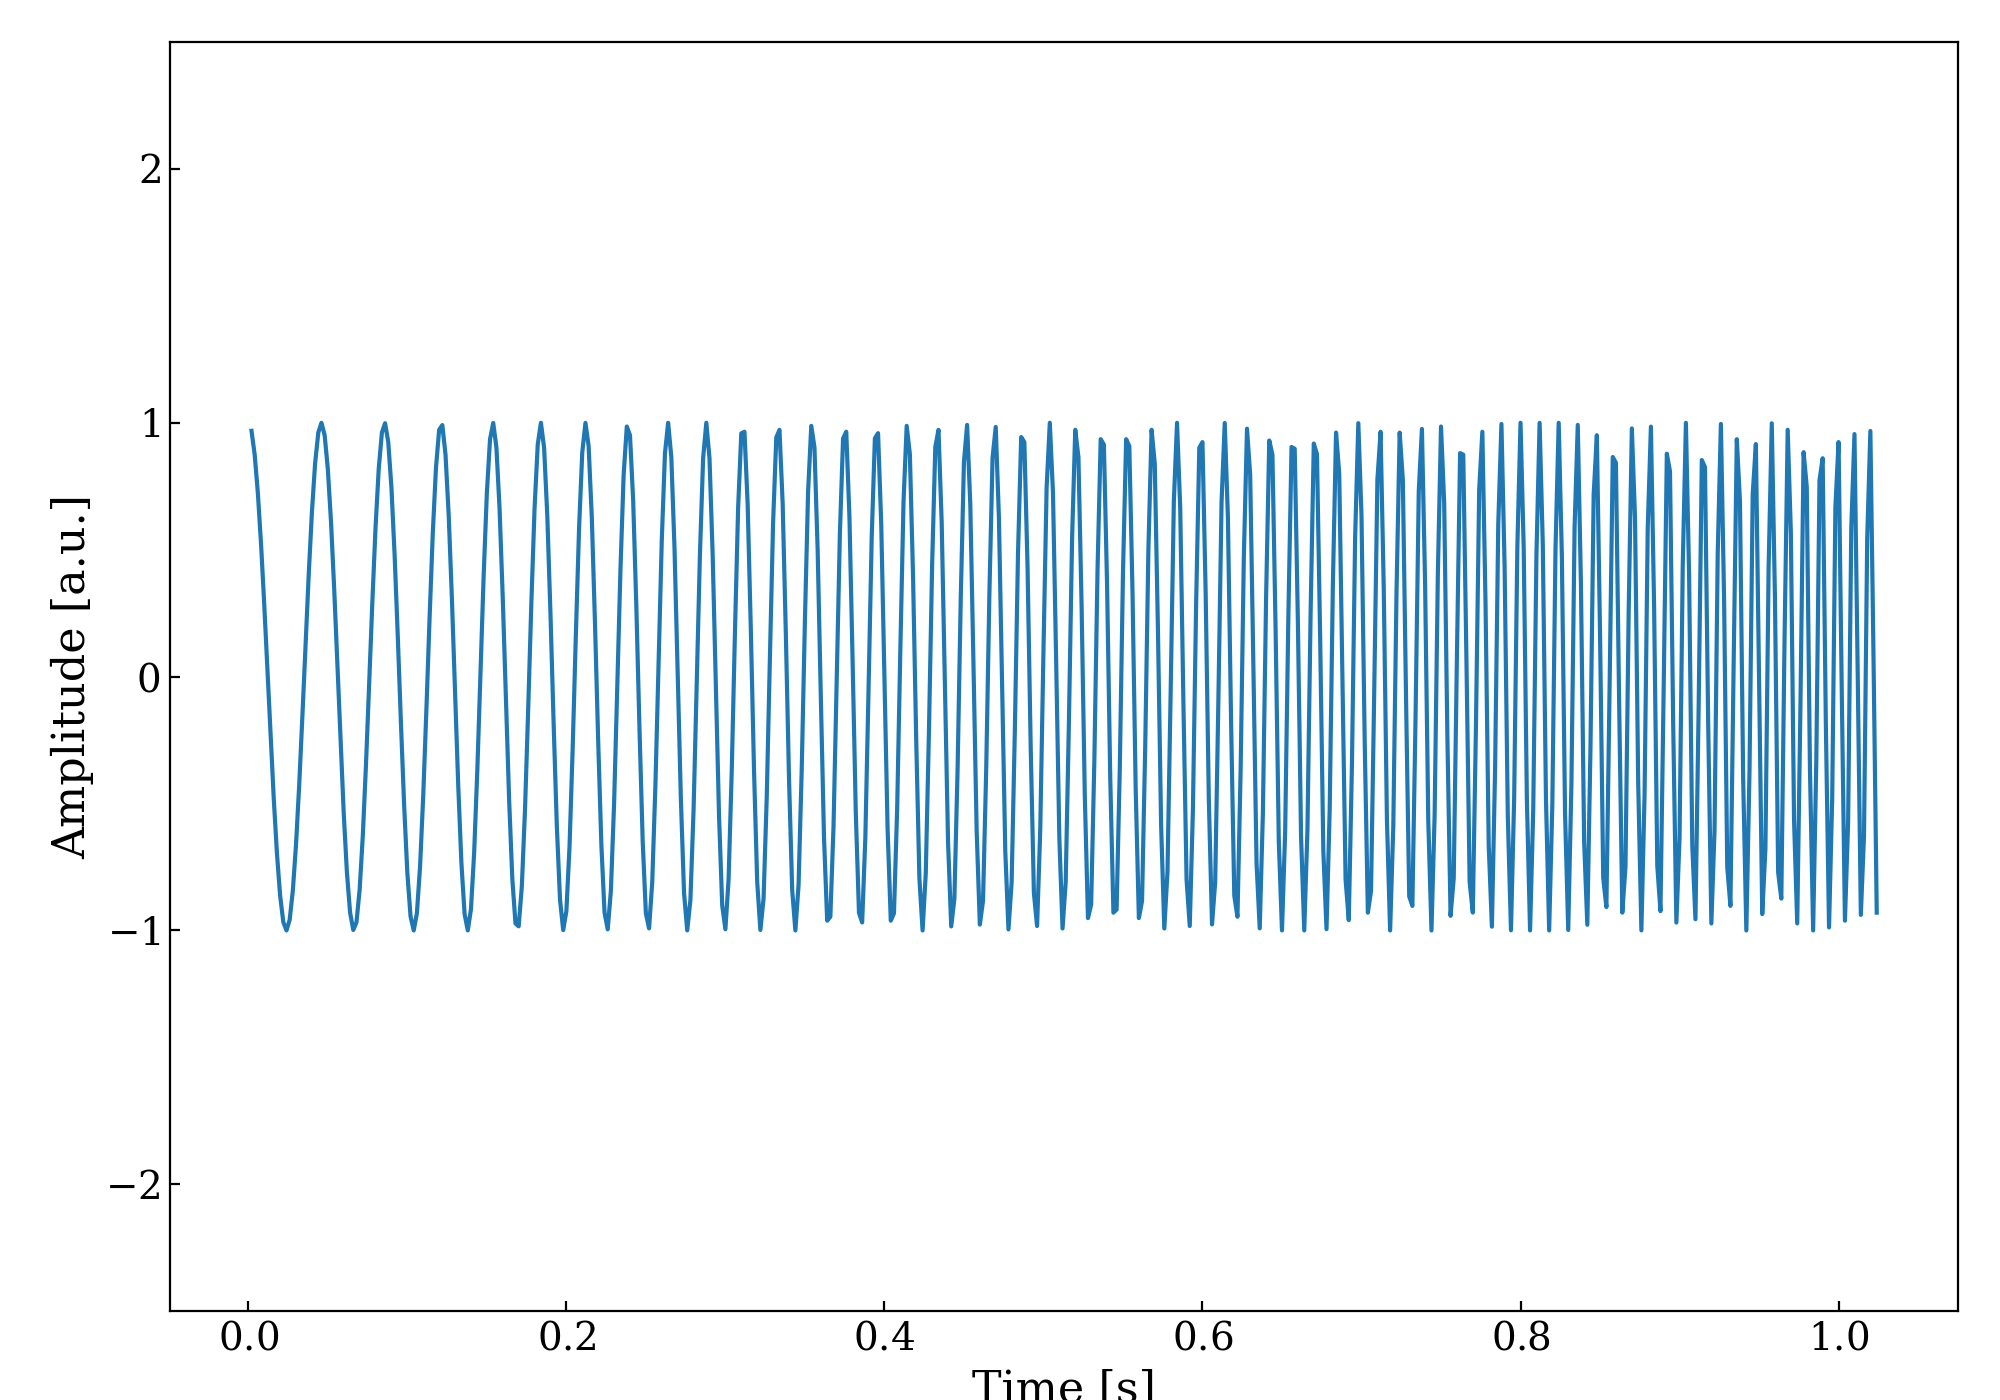
\includegraphics[width=\linewidth]{chirp.png}
    \label{fig:chirp}
\end{figure}
\pagebreak


\section{Spectrogram}

The following spectrograms of the prepared chirp signal showcase the manifestation of Heisenberg's uncertainty principle in signal analysis.

\begin{lstlisting}[caption={\textbf{Snippet for generating spectrogram with different nfft values.}}]
for nfft in [16, 32, 64, 128, 256]:
    _, wave = get_chirp(N=512)
    freqs, times, spect = signal.spectrogram(
        wave,
        fs=fs,
        window=("hamming"),
        nperseg=nfft // 2,
        nfft=nfft,
    )
\end{lstlisting}

\begin{figure}[ht!]
    \centering
    \caption{\textbf{Comparison of spectrograms of the chirp signal, with different nfft values.}}
    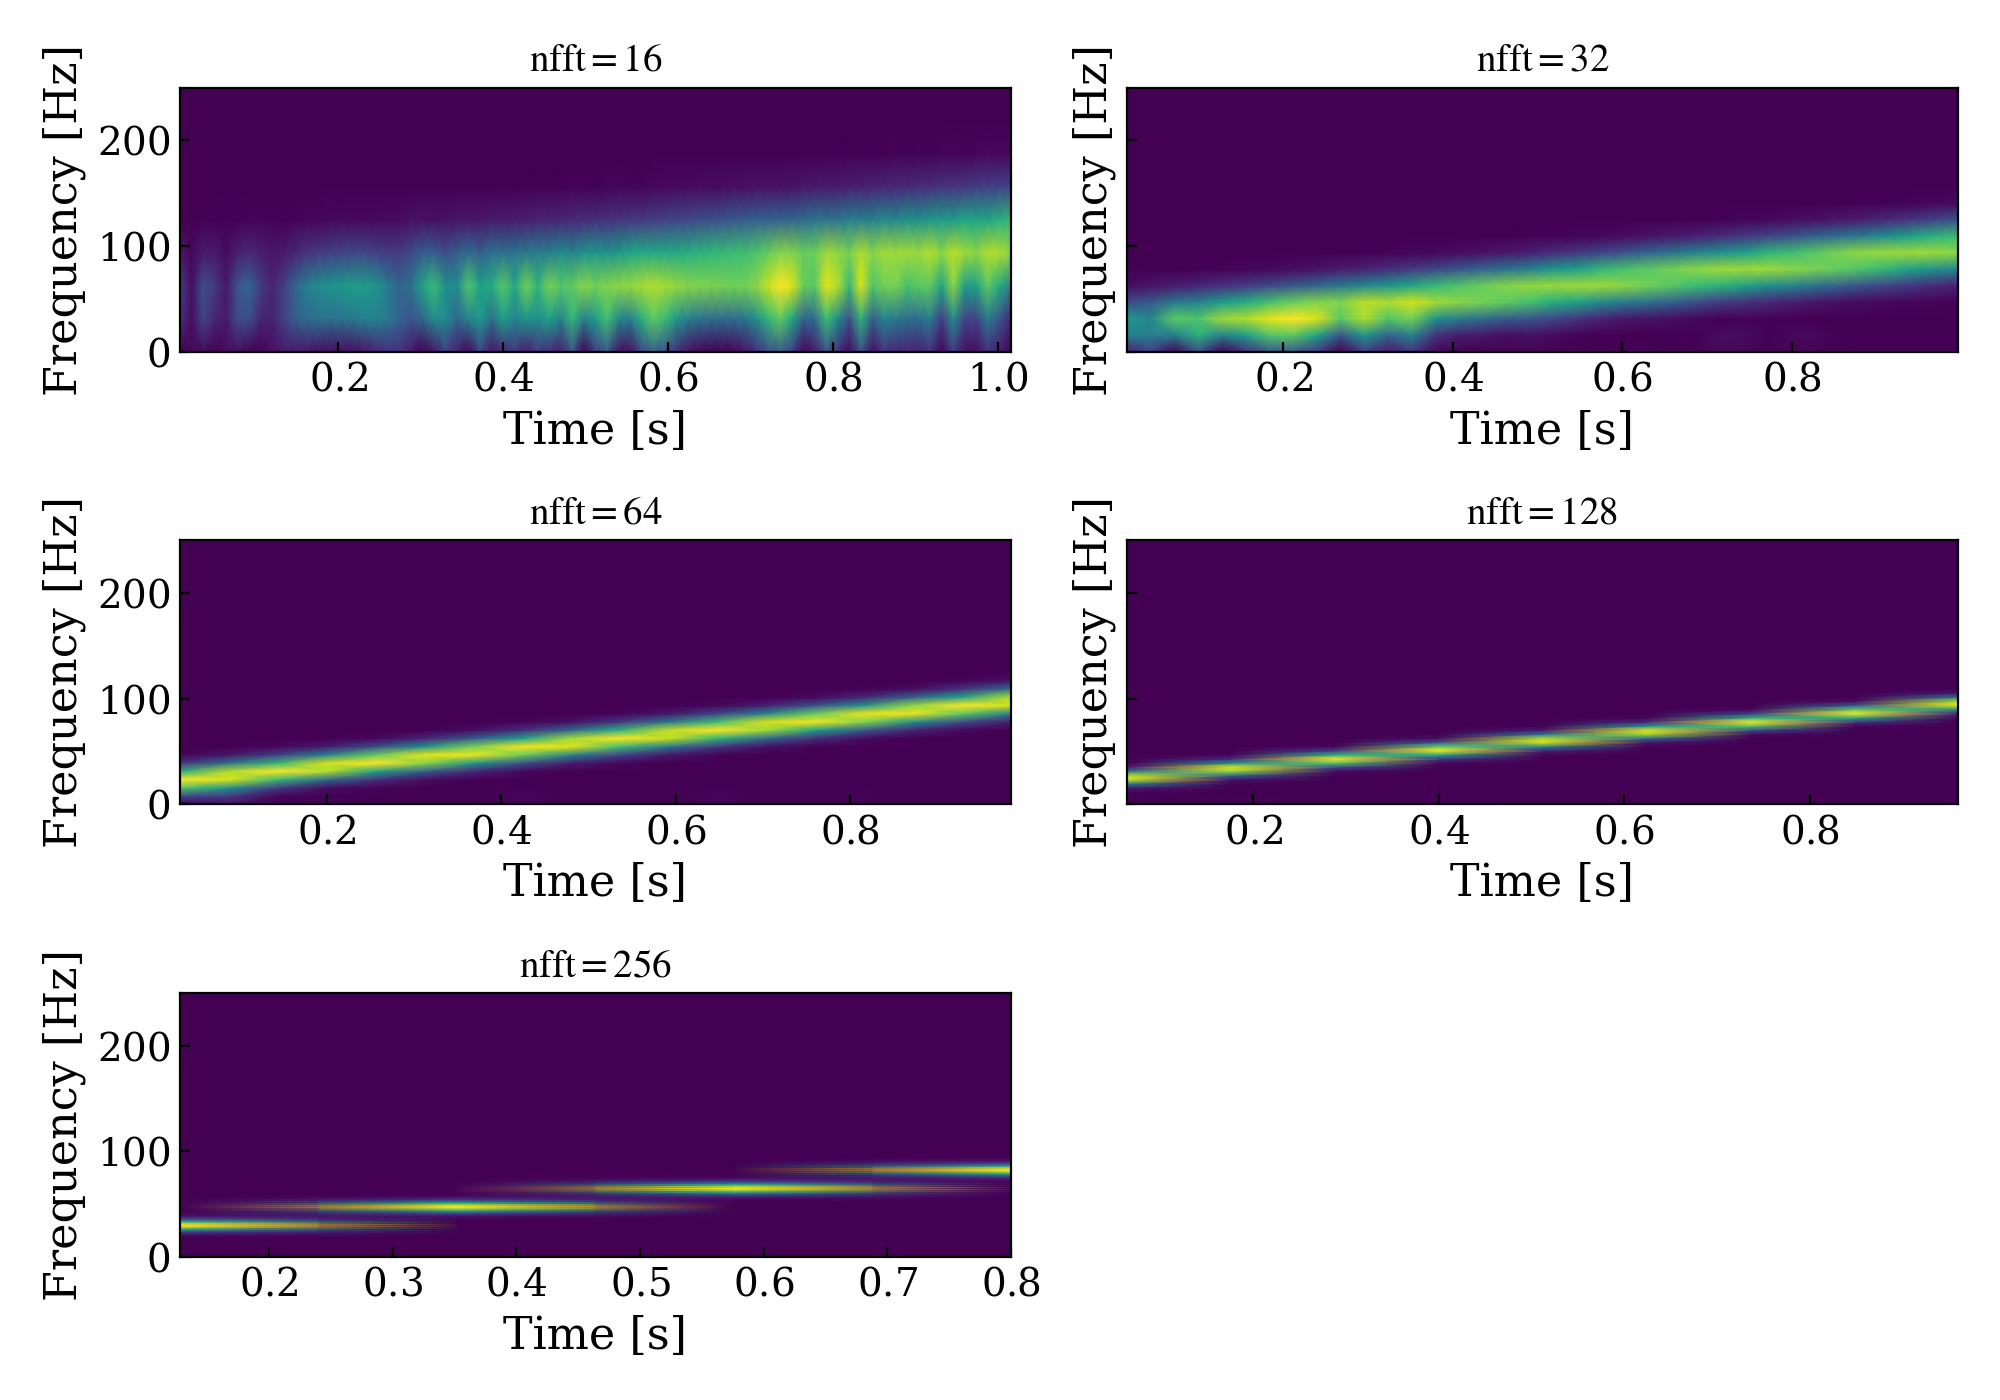
\includegraphics[width=\linewidth]{spectrogram_nfft.png}
    \label{fig:spectrogram_nfft}
\end{figure}
\pagebreak

\begin{lstlisting}[caption={\textbf{Snippet for generating spectrogram with different number of samples.}}]
for N in [1024, 2048]:
    _, wave = get_chirp(N=N)
    freqs, times, spect = signal.spectrogram(
        wave,
        fs=fs,
        window=("hamming"),
        nperseg=nfft // 2,
        nfft=nfft,
    )
\end{lstlisting}
\begin{figure}[ht!]
    \centering
    \caption{\textbf{Comparison of spectrograms of the chirp signal, with different number of samples values.}}
    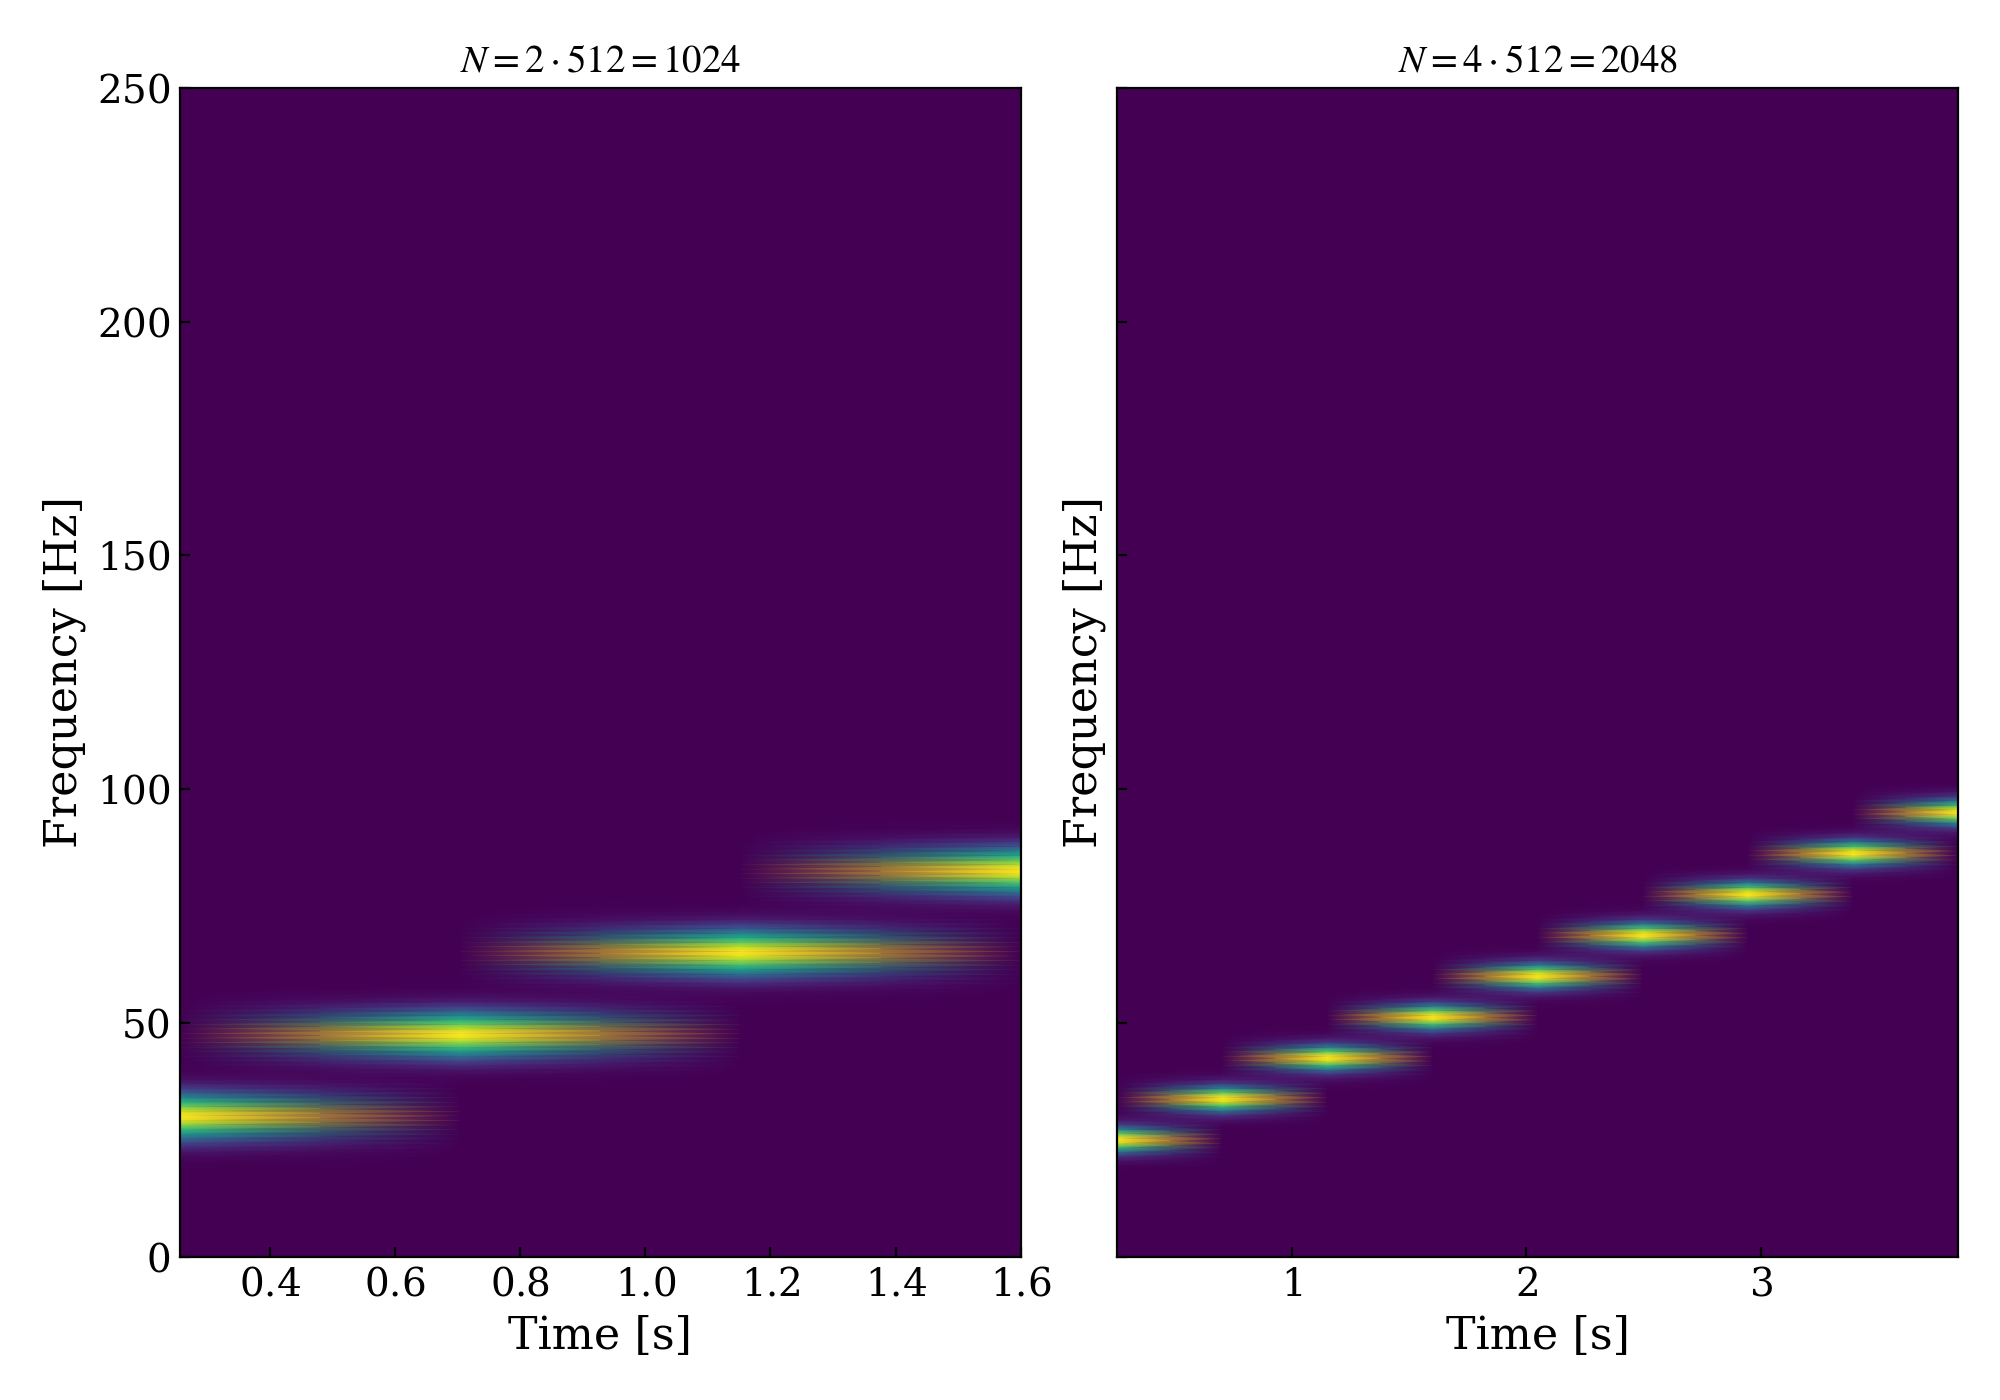
\includegraphics[width=\linewidth]{spectrogram_size.png}
    \label{fig:spectrogram_size}
\end{figure}

For the lowest analyzed value, $\text{nfft}=16$, we can observe a better resolution in the time domain. However, as one increases the value of $\text{nfft}$, the resolution in the time domain decreases in favor of the frequency domain resolution.

The above dichotomy proves the presence of the Heisenberg's uncertainty principle between time and frequency of a signal.

\pagebreak

\section{Wigner-Ville transform}

The Wigner-Ville (W-V) transform is another time-frequency analysis tool used in signal processing to study the spectral content of a signal as it varies over time.

As seen in the figure \ref{fig:wv}, W-V can offers a detailed and accurate representation of the signal's time-varying spectrum. Despite this, it greatly struggles to provide accurate results at the beginning and end of the time window.

To perform the W-V transform, the function \verb|cohen(...)|, provided with the instruction, has been used. Additionaly, to obtain an analytical function, I have used the function \verb|hilbert| from the \verb|scipy| module.

\begin{lstlisting}[caption={\textbf{Snippet for generating the W-V transform.}}]
spectrogram, frequencies, times = cohen(signal.hilbert(wave), fs)
\end{lstlisting}

\begin{figure}[ht!]
    \centering
    \caption{\textbf{W-V of the chirp signal.}}
    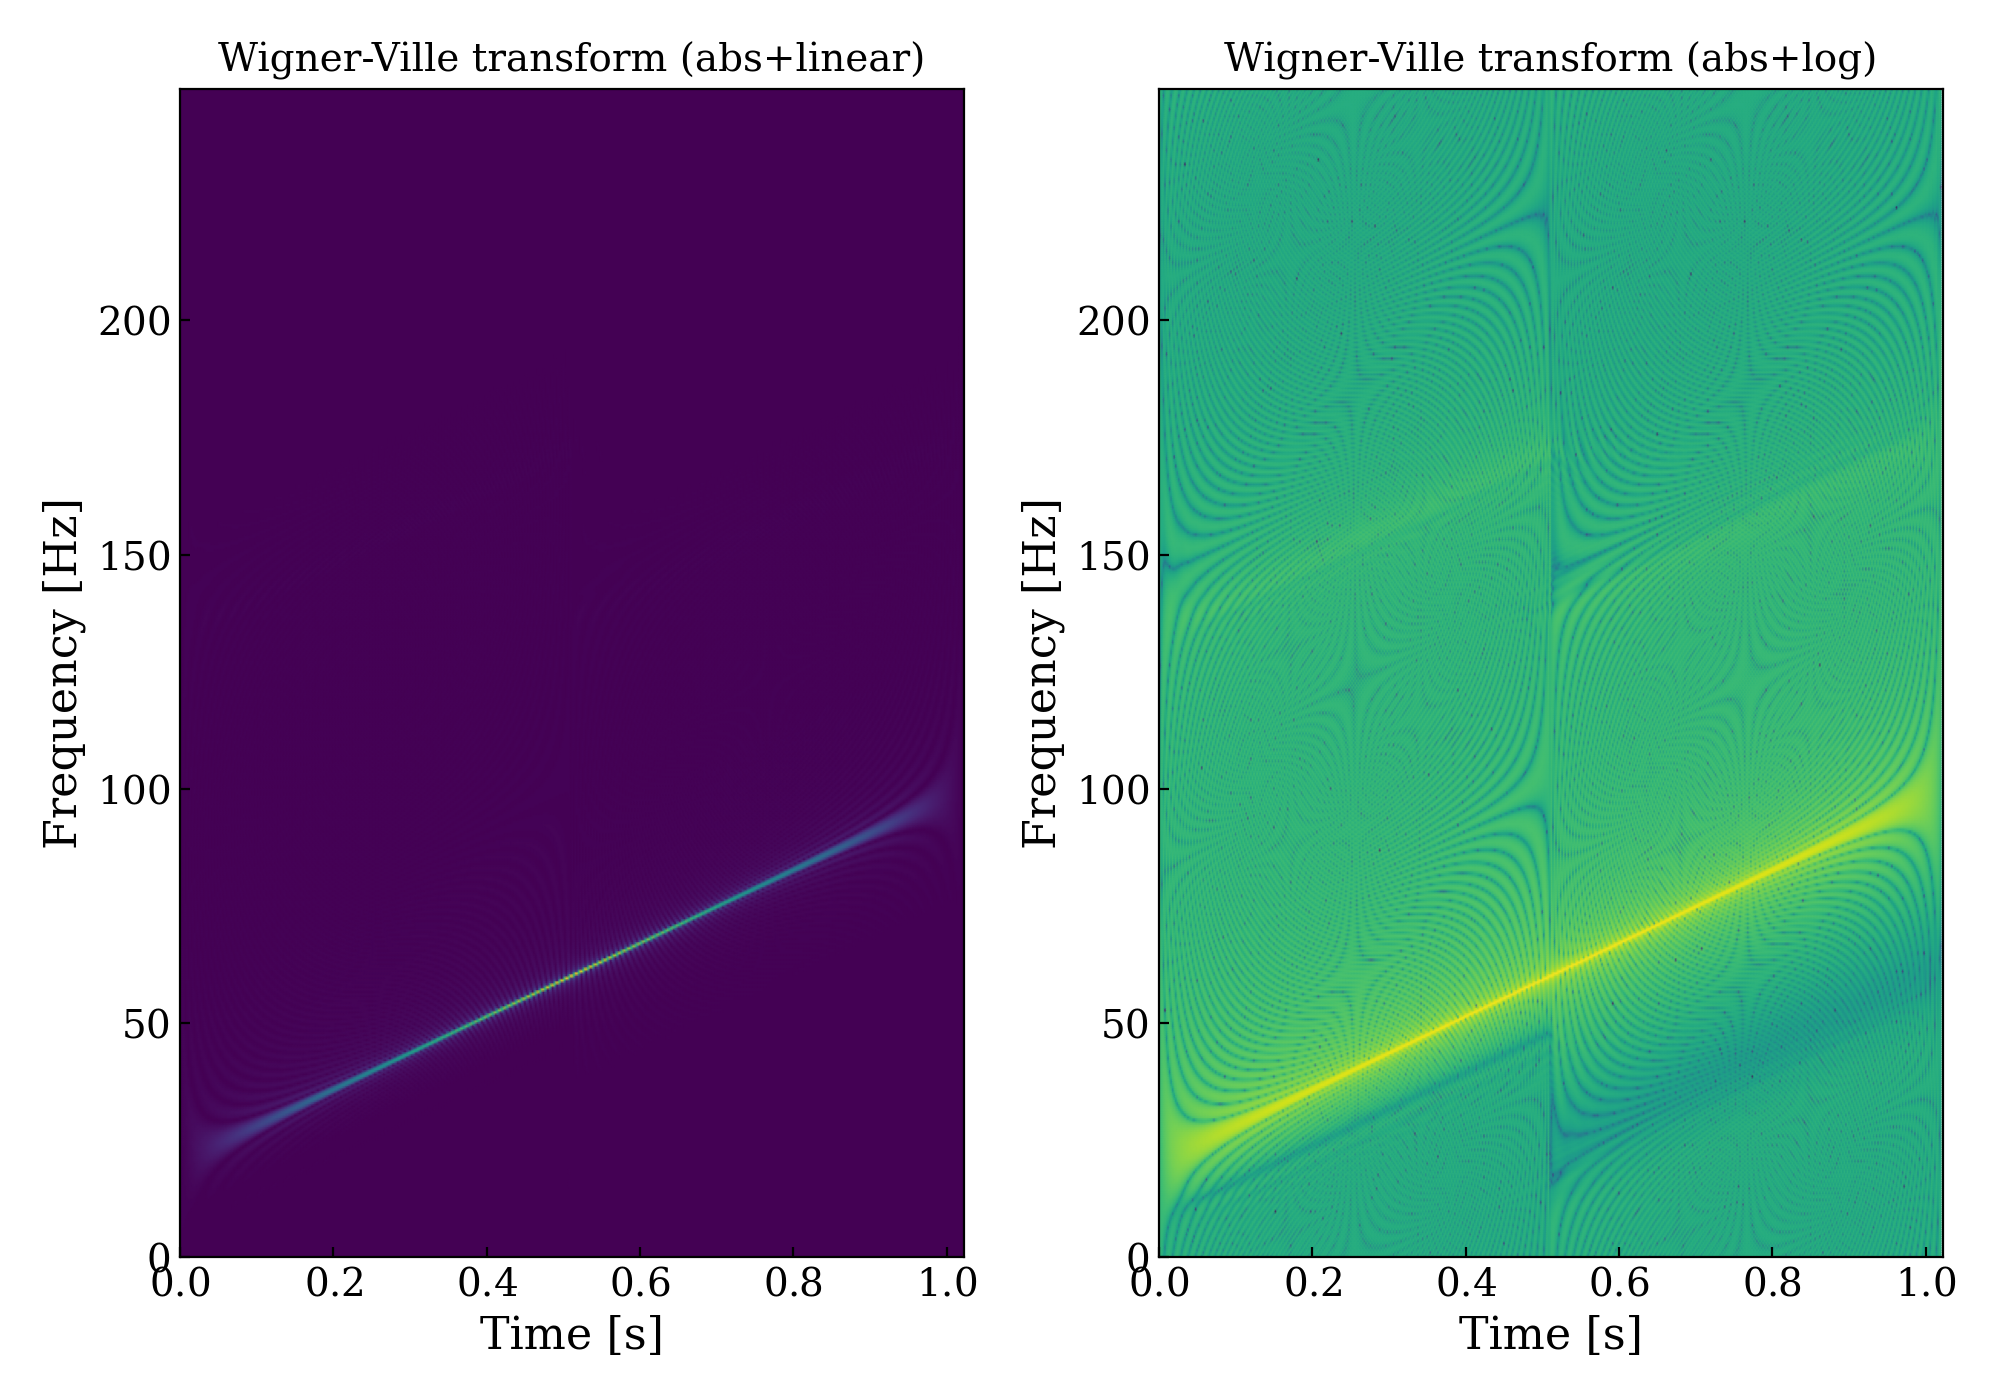
\includegraphics[width=\linewidth]{cohen.png}
    \label{fig:wv}
\end{figure}
\pagebreak


\section{W-V and STFT}

For the analysis in this section, $\text{nfft}=128$ was used.

The first plot, fig. \ref{fig:stft_f1s}, shows the W-V transform and the STFT of the chirp signal for frequencies from 200 to 500 [Hz]. Above the Nyquist frequency ($f_{nyq}=500/2=250$ [Hz]), both of the transforms exhibit aliasing, where the successive frequency components start to overlap. Such a fact makes identifying the underlying frequencies, difficult or even impossible, particularly in the W-V.

\begin{lstlisting}[caption={\textbf{Snippet for generating the STFT and W-V transform for different frequencies within specified range.}}]
for f1 in [200, 300, 400, 500]:
    time, wave = get_chirp(N=512, f1=f1)

    // W-V transform
    sxx, f, t = cohen(signal.hilbert(wave), fs)

    ...

    // STFT
    f, t, sxx = signal.spectrogram(
        wave,
        fs=fs,
        window=("hamming"),
        nperseg=nfft // 2,
        nfft=nfft,
    )
\end{lstlisting}

\begin{figure}[ht!]
    \centering
    \caption{\textbf{STFT and W-V transform for different frequencies within the range 200 to 500 [Hz].}}
    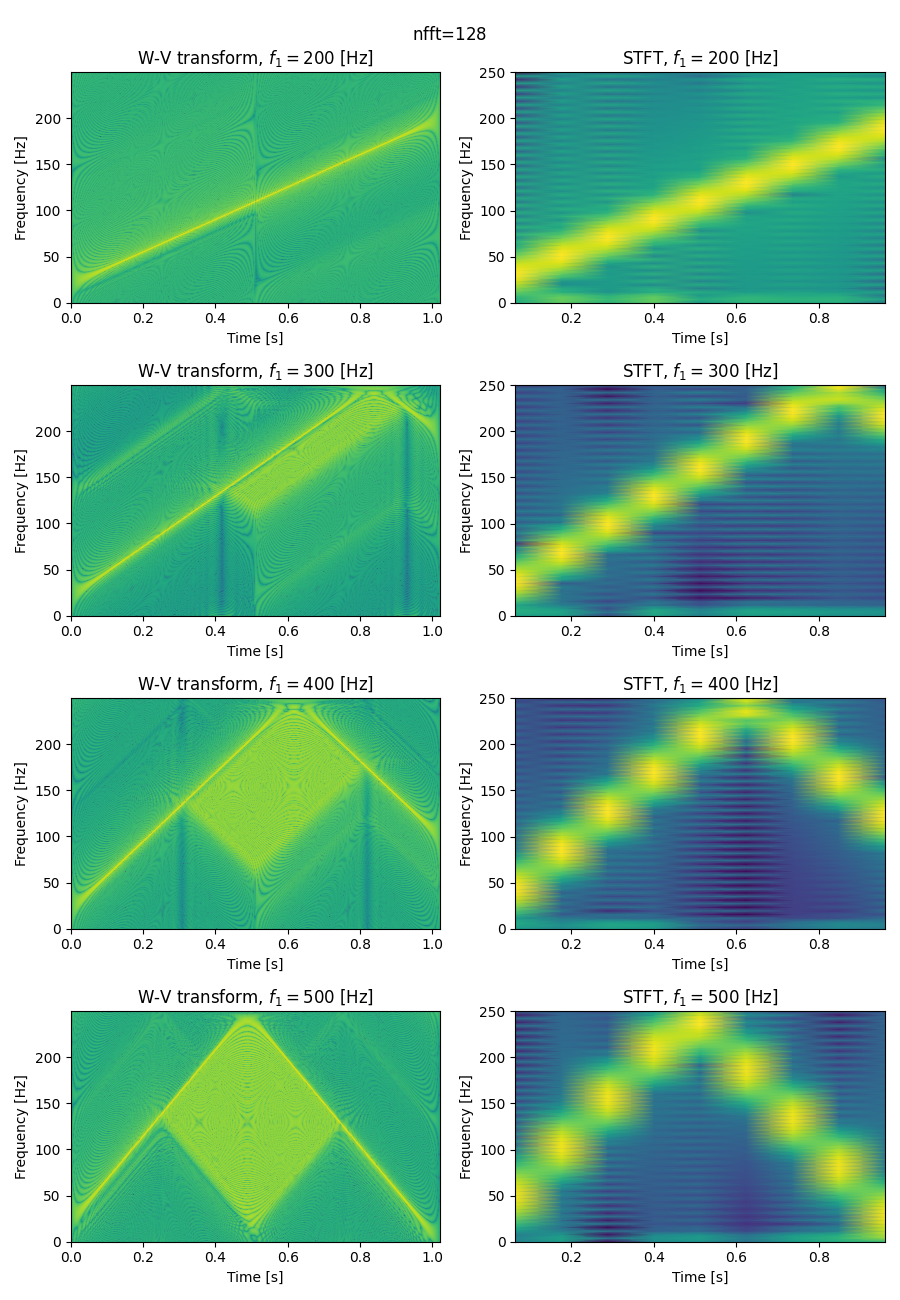
\includegraphics[width=\linewidth]{stft_f1s.png}
    \label{fig:stft_f1s}
\end{figure}
\clearpage


In fig. \ref{fig:stft_parallel}, both chirps' frequency changes align in parallel. Moreover, a third frequency component is observed, which is an average of the two.

\begin{lstlisting}[caption={\textbf{Snippet for calculating the spectrum of the sum of two chirps changing in parallel.}}]
N = 512
nfft = 128
f0 = 20
f1 = 200

time, chirp1 = get_chirp(N=N, f0=f0, f1=f1)
_, chirp2 = get_chirp(N=N, f0=2 * f0, f1=f0 + f1)
wave = chirp1 + chirp2
\end{lstlisting}

\begin{figure}[ht!]
    \centering
    \caption{\textbf{W-V transform and STFT of the sum of two chirps changing in parallel.}}
    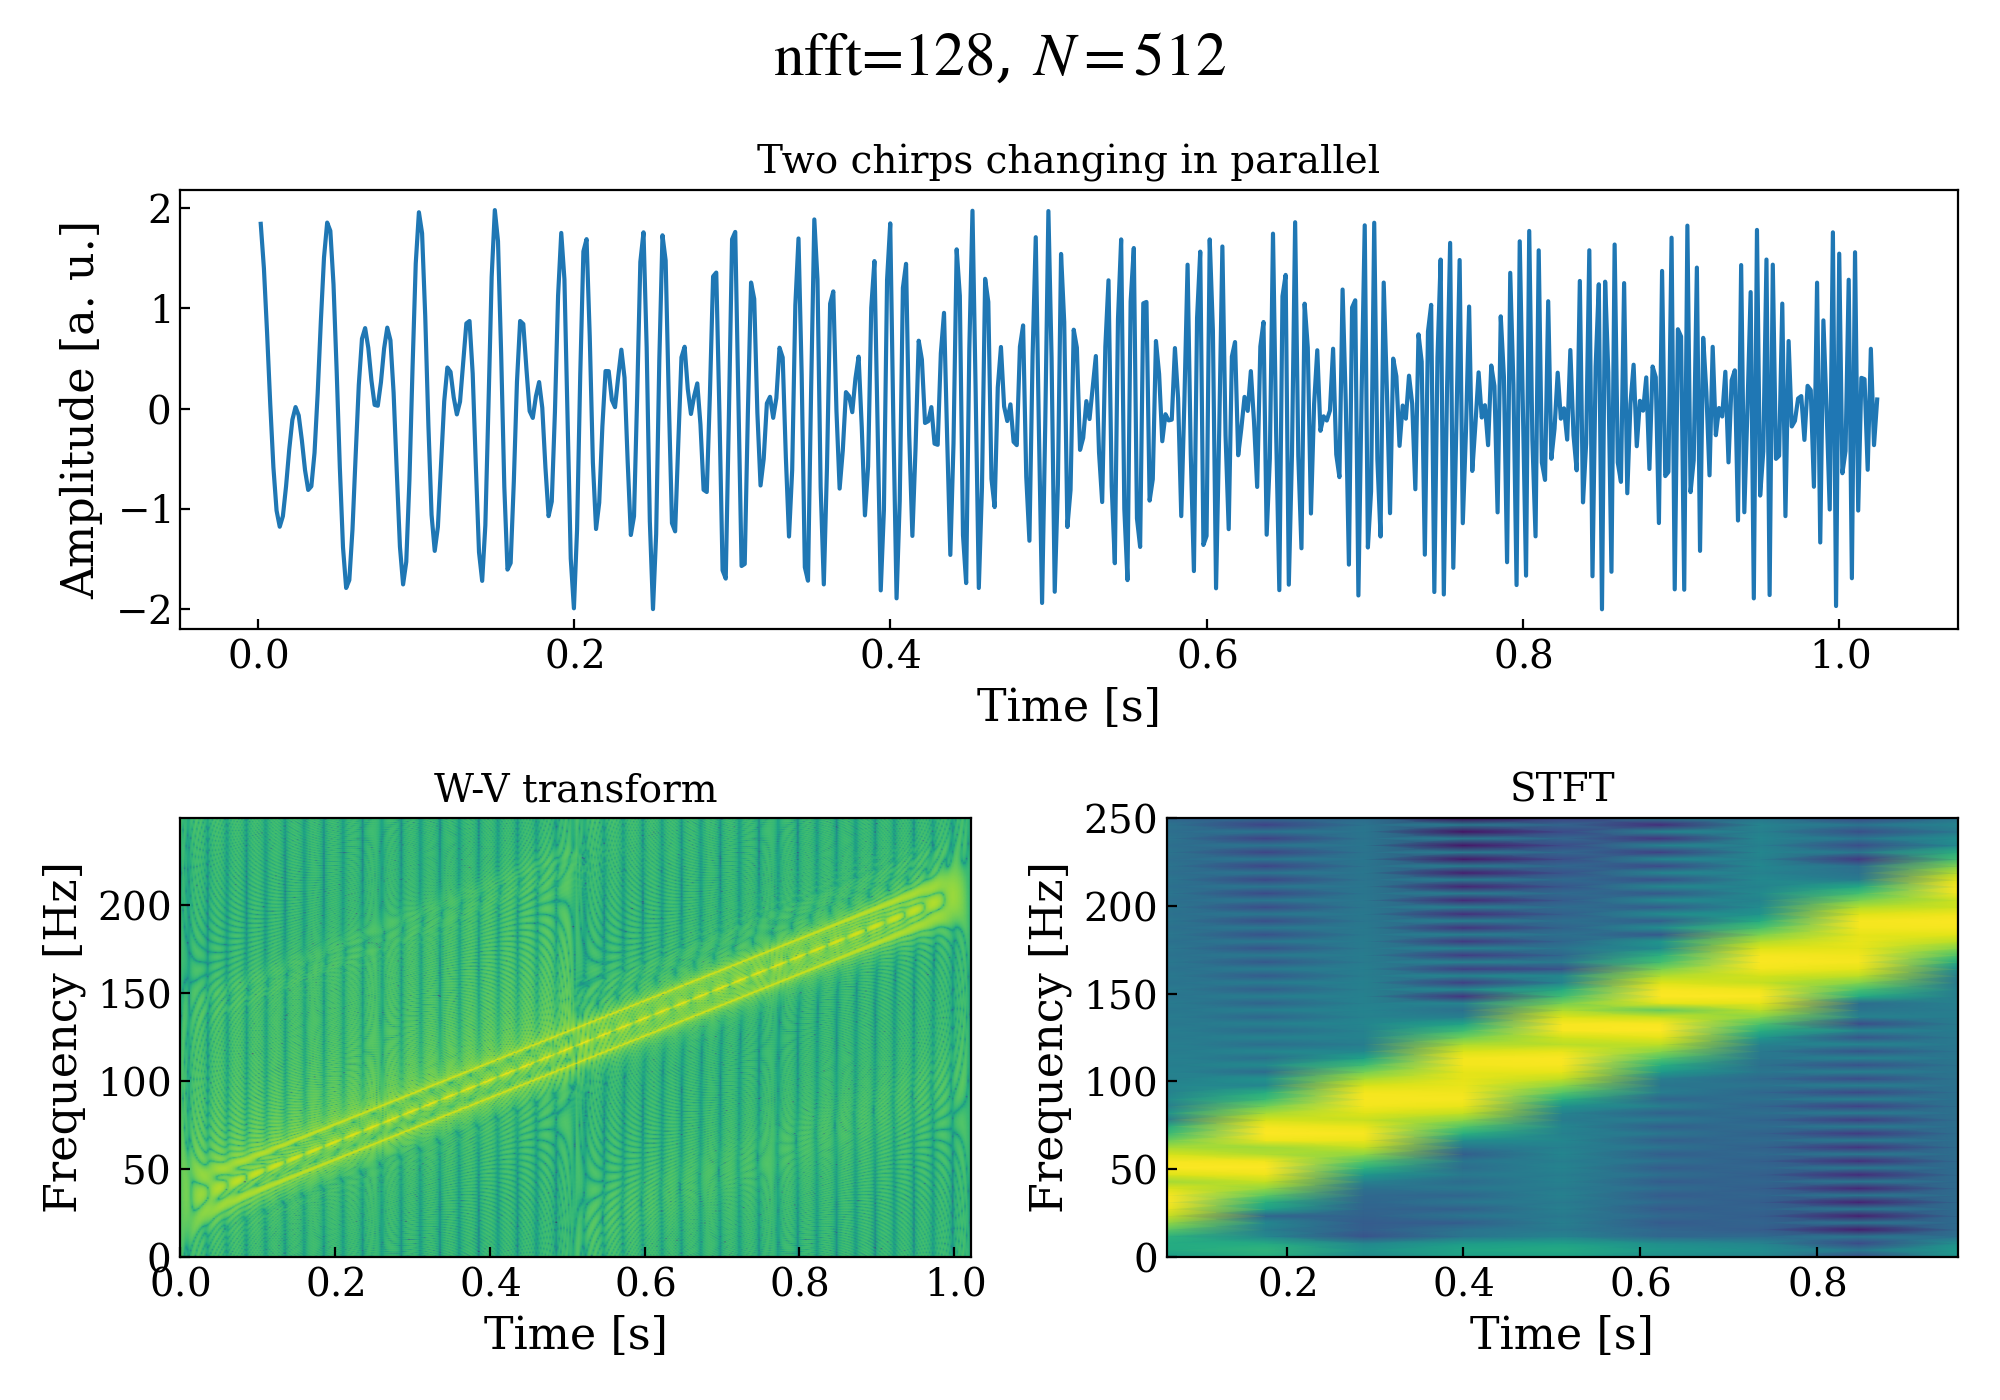
\includegraphics[width=\linewidth]{stft_parallel.png}
    \label{fig:stft_parallel}
\end{figure}
\pagebreak


As expected, in fig. \ref{fig:stft_nonparallel}, chirps' frequencies do not change in parallel, which manifests itself as multiple intersecting lines.

\begin{lstlisting}[caption={\textbf{Snippet for calculating the spectrum of the sum of two chirps changing in parallel.}}]
N = 512
nfft = 128
f0 = 20
f1 = 200

time, chirp1 = get_chirp(N=N, f0=f0, f1=f1)
_, chirp2 = get_chirp(N=N, f0=2 * f0, f1=2 * f1)
wave = chirp1 + chirp2
\end{lstlisting}

\begin{figure}[ht!]
    \centering
    \caption{\textbf{W-V transform and STFT of the sum of two chirps changing not in parallel.}}
    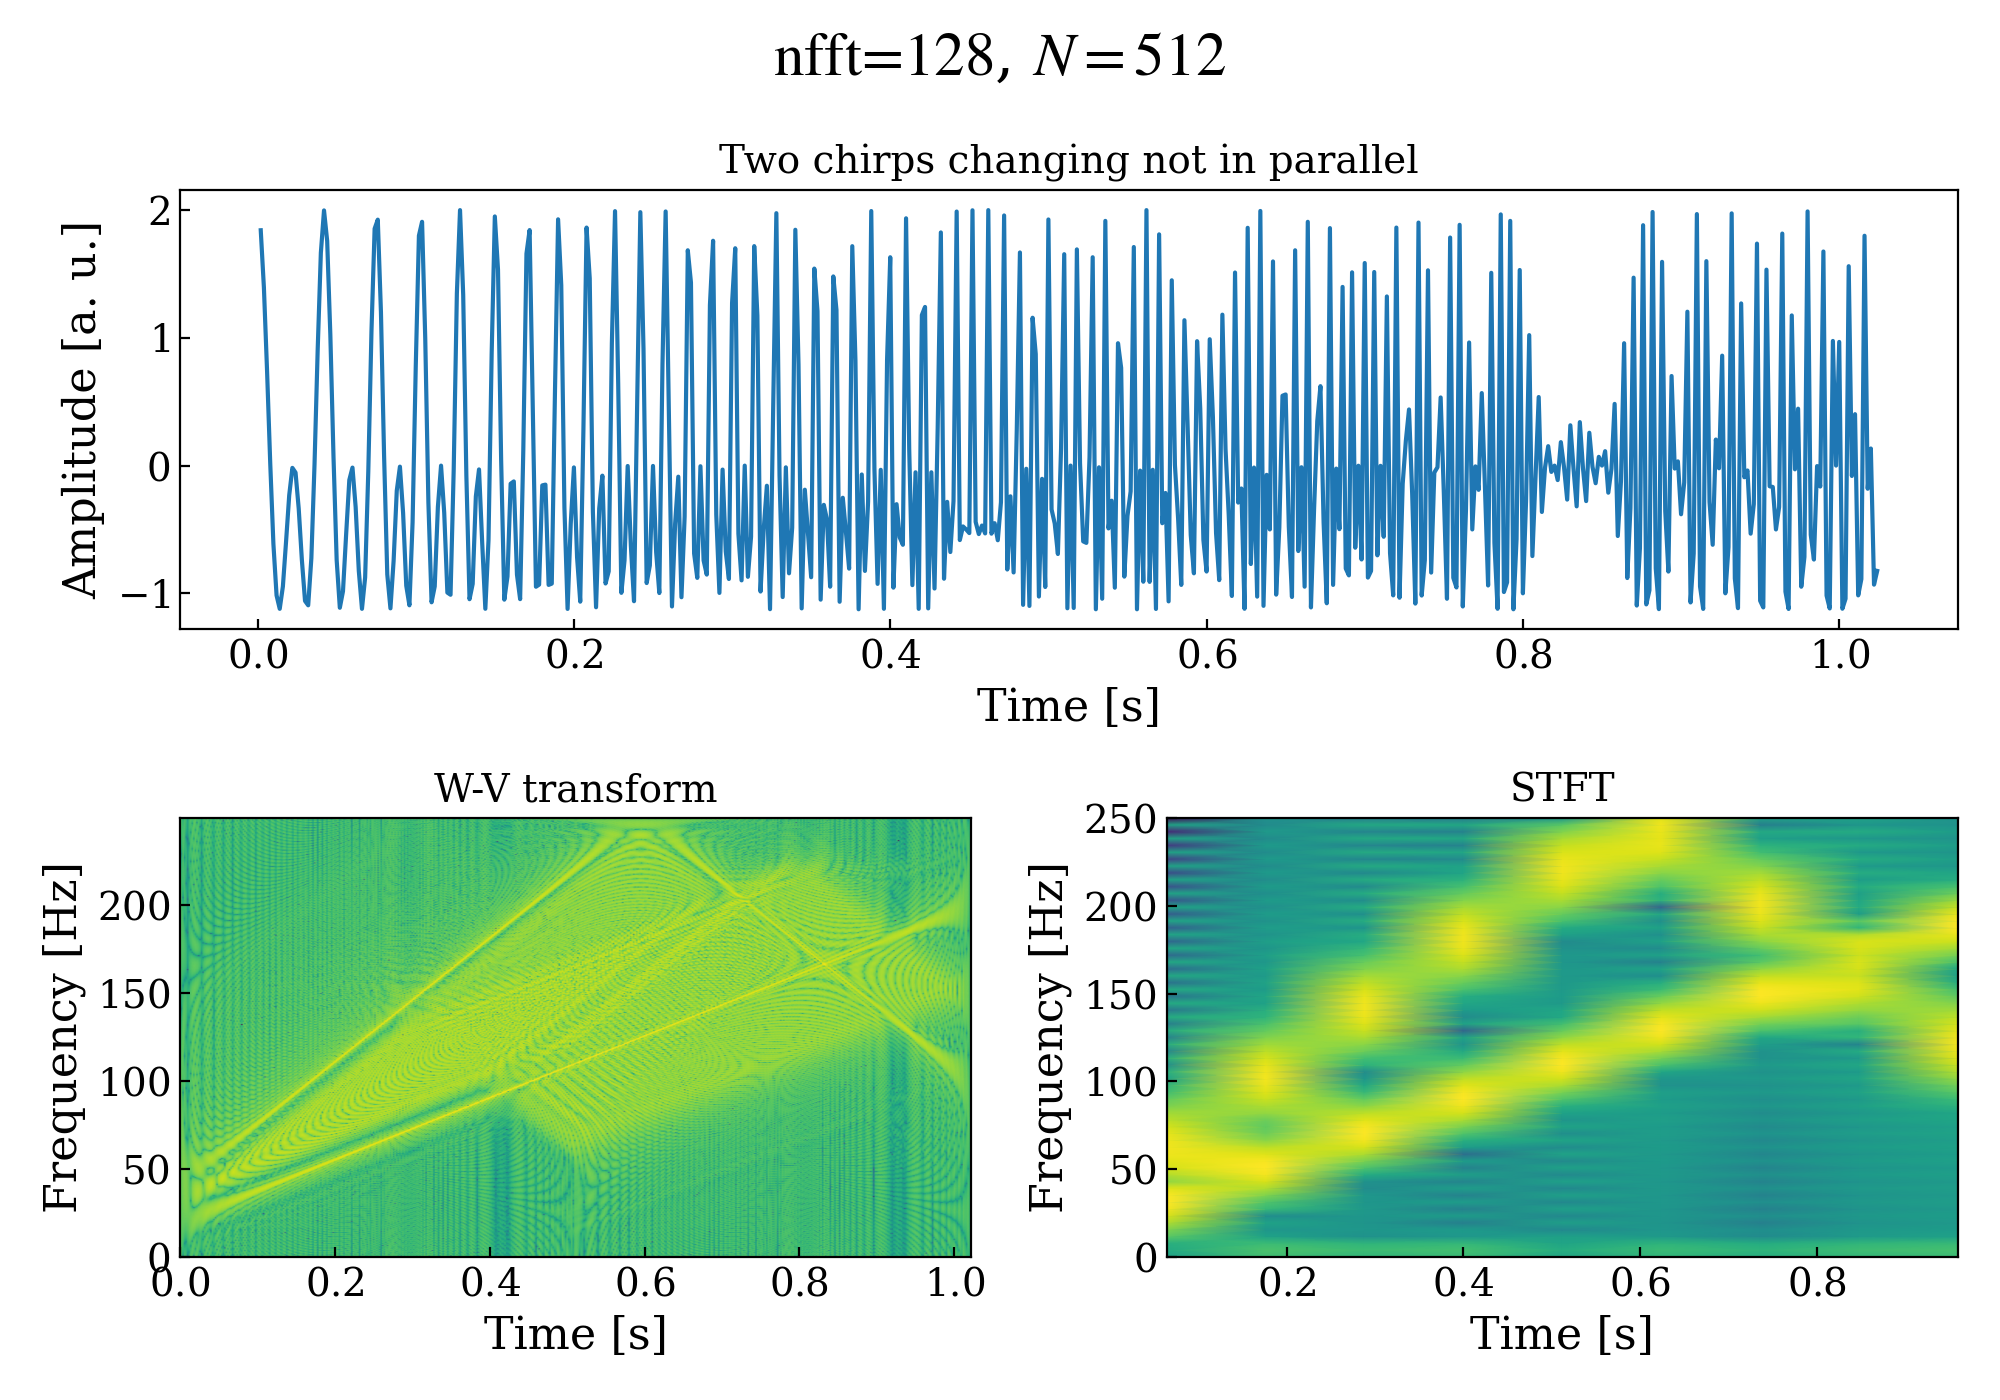
\includegraphics[width=\linewidth]{stft_nonparallel.png}
    \label{fig:stft_nonparallel}
\end{figure}
\pagebreak


\section{Conclusion}

In conclusion, the report explores time-frequency analysis techniques, focusing on Short-time Fourier Transform (STFT) and Wigner-Ville transform. Analysis of chirp signals illustrates the manifestation of Heisenberg's uncertainty principle. Despite limitations, both transforms provide valuable insights into signal processing, aiding in understanding time-varying spectral content.

The entire code for generating the data and plots can be found at:

\url{https://github.com/davkk/signal-analysis/tree/main/sat/lab03}

\begin{thebibliography}{9}
\bibitem{scipychirp} https://docs.scipy.org/doc/scipy/reference/generated/scipy.signal.chirp.html
\end{thebibliography}

\end{document}
